\documentclass[11pt,oneside,a4paper]{article} %draft
\usepackage[latin1]{inputenc}
%\usepackage{a4wide}
%\usepackage{beton}
%\usepackage{amsmath}
\usepackage{hyperref}
\usepackage{graphicx}
\usepackage{color}
\usepackage{amssymb}
\usepackage{hyperref}
\usepackage{cancel}
\usepackage{verbatim}
\usepackage{latexsym}
\usepackage[spanish]{babel}
\usepackage{upgreek}
\usepackage{pdfpages}
\usepackage[a4paper,margin=2cm]{geometry}
%\pagestyle{empty}

\begin{document}
\parindent 0mm
\parskip 4mm

\topmargin 10mm
\textheight 228mm

%\AddToShipoutPicture{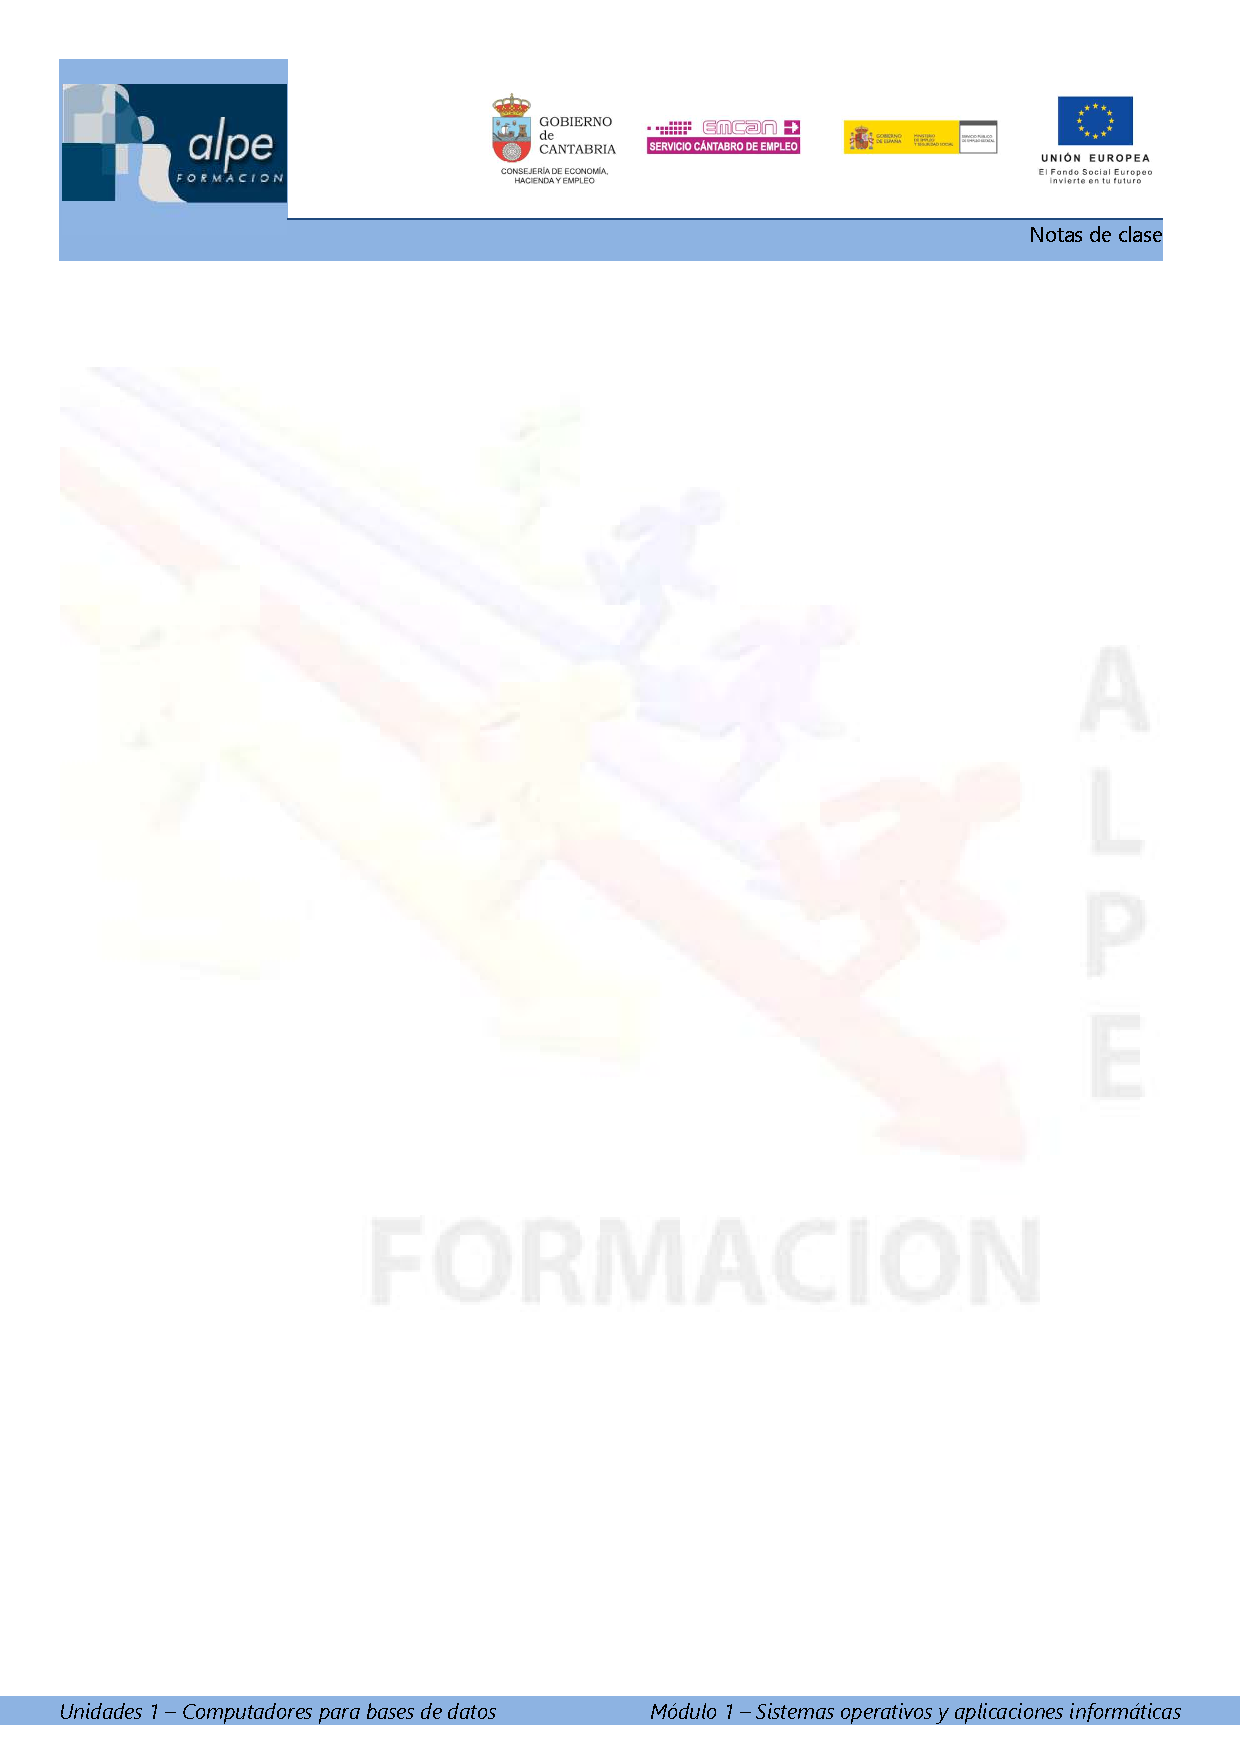
\includegraphics[width=\paperwidth,height=\paperheight,keepaspectratio]{fondo_m1}}

\newcommand{\hs}{\hspace{1mm}}
\newcommand{\G}{ \textrm{\c{G}}}
\newcommand{\ljoin}{ \ltimes }
\newcommand{\rjoin}{ \rtimes }
\newcommand{\fjoin}{ ]\mkern-9mu\times\mkern-9mu [ }
\newcommand{\tbl}[1]{$#1$}
\newcommand{\cmp}[1]{$#1$}

%\tableofcontents
%\newpage
%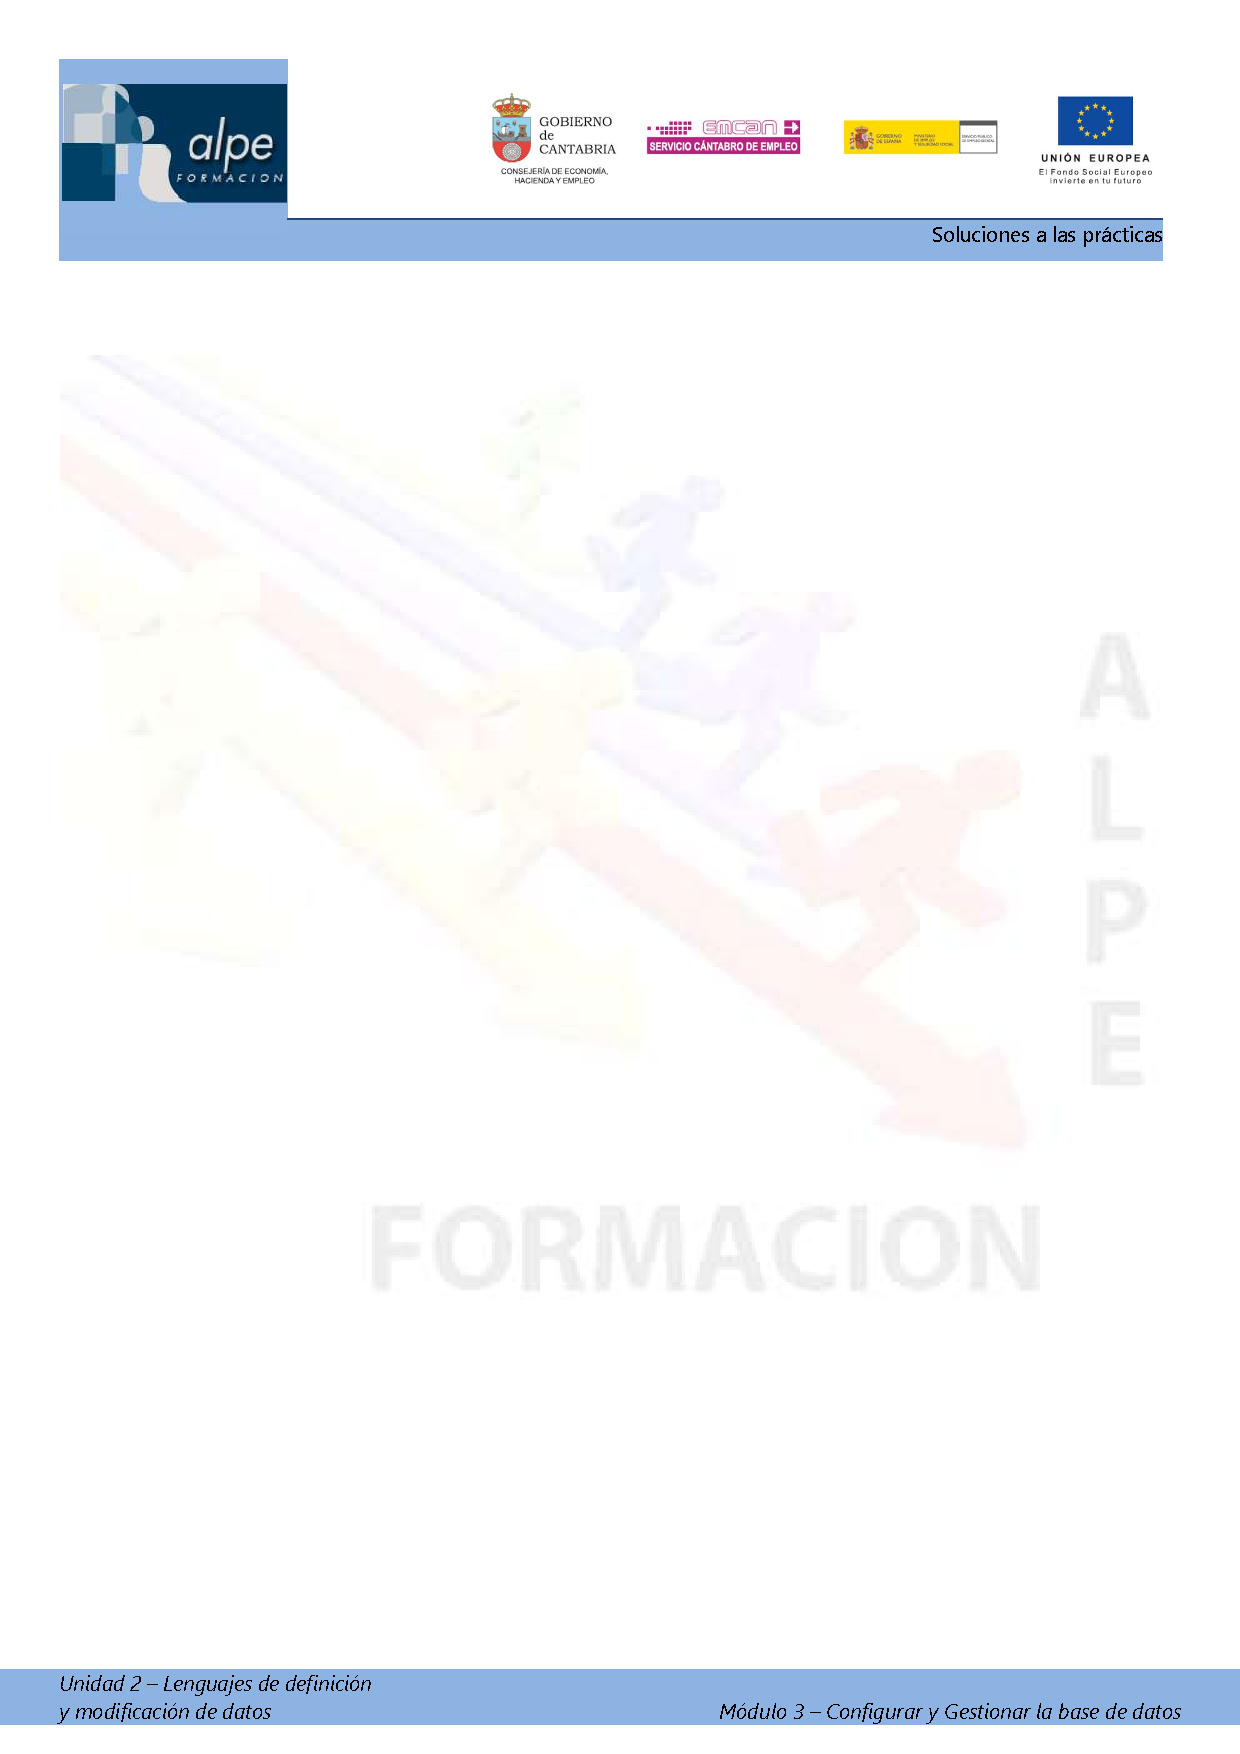
\includepdf[pages=-,offset=0mm 0]{fondo}
%\ClearShipoutPicture
%\includepdf[pages=-,offset=14mm 0]{Ord_201_18783_25032015_fdo}

	\centering



$2^3 = 8$

$2^{-3} = 1/8 = 0.125$

2E3 = $2*10^3 = 2000$

2E-3 $= 2*10^{-3} = 2/1000 = 0.002$

$2^4 * 2^6 = 2^{10}$ = 1K

$2^11 = 2 * 2^{10}$= 2K

KM = G

mG = M

$\frac{\textnormal{KM}}{\textnormal{M}}$=K

$1/M = \upmu$
$1/G = n$
	

1 operaci�n * $\frac{1s}{
	\textnormal{2 G operaciones}
	}$ = $\frac{1}{2}$ ns $\frac{1000ps}{1ns} $ = 500 ps


\begin{table}[hpbt]
	\centering
		\begin{tabular}{cc}
$2^0$	& 1\\
$2^1$	& 2\\
$2^2$	& 4\\
$2^3$	& 8\\
$2^4$	& 16\\
$2^5$	& 32\\
$2^6$	& 64\\
$2^7$	& 128\\
$2^8$	& 256\\
$2^9$	& 512\\
$2^{10}$	& 1024 = 1K\\
$2^{11}$	& 2048\\
$2^{12}$	& 4096\\
$2^{13}$	& 8192\\
$2^{20}$	& 1M\\
$2^{30}$	& 1G\\
$2^{40}$	& 1T\\
$2^{50}$	& 1P\\
		\end{tabular}
	\caption{Tabla de potencias de dos}
	\label{tab:TablaDePotenciaDeDos}
\end{table}


\newpage

\begin{table}[hpbt]
	\centering
		\begin{tabular}{|c|c|c|c|}\hline
Peta &P & $10^{15}$	& $2^{50}$ \\\hline
Tera & T & $10^{12}$	& $2^{40}$ \\\hline		
Giga &G & $10^9$	& $2^{30}$ \\\hline
Mega&M & $10^6$	& $2^{20}$ \\\hline
Kilo&K & $10^3$	& $2^{10}$ \\\hline
mili&m & $10^{-3}$	& $2^{-10}$ \\\hline
micro&$\upmu$ & $10^{-6}$	& $2^{-20}$ \\\hline
nano&n & $10^{-9}$	& $2^{-30}$ \\\hline
pico&p & $10^{-12}$	& $2^{-40}$ \\\hline
femto&f & $10^{-15}$	& $2^{-50}$ \\\hline
		\end{tabular}
	\caption{Multiplicadores y divisores}
	\label{tab:MultiplicadoresYDivisores}
\end{table}




\begin{table}[hpbt]
	\centering
		\begin{tabular}{rrrr}
DEC&BIN&OCT&HEX\\
00&0000&00&0\\
01&0001&01&1\\
02&0010&02&2\\
03&0011&03&3\\
04&0100&04&4\\
05&0101&05&5\\
06&0110&06&6\\
07&0111&07&7\\
08&1000&10&8\\
09&1001&11&9\\
10&1010&12&A\\
11&1011&13&B\\
12&1100&14&C\\
13&1101&15&D\\
14&1110&16&E\\
15&1111&17&F\\
16& 1 0000&20&10\\
		\end{tabular}
	\caption{Sistemas de numeraci�n}
	\label{tab:SistemasDeNumeracion}
\end{table}



\end{document}